% !TEX root = ../../../main.tex
% 所属：第一部分：单变量分析学 / 第10章：一些定积分的问题
% 节：10.4 积分不等式~~二 
% 正文按原文件顺序保存；由 ../chapter10.tex 调用。
\section{积分不等式~~二 }
\begin{proposition}
（Cauchy-Schwarz 不等式）

若 $f,g \in \mathcal{R}[a,b]$，则有
\[\left( \int_{a}^{b} f g \dd x \right)^2
\leq 
\int_{a}^{b} f^2 \dd x \cdot \int_{a}^{b} g^2 \dd x\]

当且仅当存在常数 $k$，使得 $g(x)=k f(x)$ 或 $f(x)=k g(x)$ 时，等号成立。
\end{proposition}
\begin{proof}
	法一：$\forall \lambda \in \mathbb{R}$，有$(f(x)+\lambda g(x))^2 \geqslant 0$，则
	\[
	\int_{a}^{b} (f+\lambda g)^2 \dd x \geqslant 0
	\]
	也即 $\forall \lambda \in \mathbb{R}$
	\begin{align*}
		\int_{a}^{b} (f+\lambda g)^2 \dd x
		&= \int_{a}^{b} f^2 \dd x + 2\lambda \int_{a}^{b} fg \dd x + \lambda^2 \int_{a}^{b} g^2 \dd x \geqslant 0
	\end{align*}
	上述是关于 $\lambda$ 的一元二次多项式，其恒非负故判别式 $\Delta \leqslant 0$，故
	\[
	\Delta = \left( 2\int_{a}^{b} fg \dd x \right)^2 - 4 \int_{a}^{b} f^2 \dd x \int_{a}^{b} g^2 \dd x \leqslant 0
	\]
	也即
	\[
	\left( \int_{a}^{b} fg \dd x \right)^2 \leqslant \int_{a}^{b} f^2 \dd x \cdot \int_{a}^{b} g^2 \dd x
	\]
	
	法二：令
	\[
	F(x) = \int_{a}^{x} f^2 \dd t \int_{a}^{x} g^2 \dd t - \left[ \int_{a}^{x} fg \dd t \right]^2
	\]
	显然 $F(a) = 0$
	\begin{align*}
		F'(x) &= f^2(x) \int_{a}^{x} g^2 \dd t + g^2(x) \int_{a}^{x} f^2 \dd t - 2f(x)g(x) \int_{a}^{x} fg \dd t \\
		&= \int_{a}^{x} \left[ f(x)g(t) - g(x)f(t) \right]^2 \dd t \geqslant 0
	\end{align*}
	$F(x)$ 在 $x \geqslant a$ 上单调递增，因此 $F(x) \geqslant F(a) = 0$，于是 $F(b) \geqslant F(a) = 0$
\end{proof}

\begin{problem}
	已知 $f(x)\geqslant 0$，在 $[a,b]$ 上连续，$\displaystyle\int_a^b f(x)\dd x=1$，$k$ 为任意实数，证明：
	\[
	\left(\int_a^b f(x)\cos kx\dd x\right)^2+
	\left(\int_a^b f(x)\sin kx\dd x\right)^2\leqslant 1.
	\]
\end{problem}

\begin{proof}
	由 Cauchy-Schwarz 不等式，
	\[
	\left(\int_a^b f(x)\cos kx\dd x\right)^2
	=\left(\int_a^b \sqrt{f(x)}\sqrt{f(x)}\cos kx\dd x\right)^2
	\leqslant \int_a^b f(x)\dd x\int_a^b f(x)\cos^2kx\dd x.
	\]
	同理，
	\[
	\left(\int_a^b f(x)\sin kx\dd x\right)^2
	\leqslant \int_a^b f(x)\dd x\int_a^b f(x)\sin^2kx\dd x.
	\]
	两式相加，并利用 $\displaystyle\int_a^b f(x)\dd x=1$，得
	\[
	\left(\int_a^b f(x)\cos kx\dd x\right)^2+
	\left(\int_a^b f(x)\sin kx\dd x\right)^2
	\leqslant \int_a^b f(x)\dd x=1.
	\]
\end{proof}

\begin{problem}
	设实函数 $f(x)$ 及其一阶导数在 $[a,b]$ 上连续，且 $f(a)=0$，证明：
	\[
	\max_{a\leqslant x\leqslant b}|f(x)|
	\leqslant \left((b-a)\int_a^b |f'(t)|^2\dd t\right)^{\frac12},
	\]
	并且
	\[
	\int_a^b f^2(t)\dd t
	\leqslant \frac12(b-a)^2\int_a^b |f'(t)|^2\dd t.
	\]
\end{problem}

\begin{proof}
	对任意 $x\in[a,b]$，有
	\[
	f(x)=\int_a^x f'(t)\dd t.
	\]
	由 Cauchy-Schwarz 不等式，
	\[
	|f(x)|\leqslant \int_a^x |f'(t)|\dd t
	\leqslant \sqrt{x-a}\left(\int_a^x |f'(t)|^2\dd t\right)^{\frac12}
	\leqslant \left((b-a)\int_a^b |f'(t)|^2\dd t\right)^{\frac12}.
	\]
	于是第一式成立。
	又
	\[
	f^2(x)\leqslant (x-a)\int_a^b |f'(t)|^2\dd t,
	\]
	两边在 $[a,b]$ 上积分，得
	\[
	\int_a^b f^2(x)\dd x
	\leqslant \int_a^b (x-a)\dd x\int_a^b |f'(t)|^2\dd t
	=\frac12(b-a)^2\int_a^b |f'(t)|^2\dd t.
	\]
\end{proof}

\begin{problem}
	设 $f(x)$ 在 $[0,1]$ 上连续，且 $\displaystyle\int_0^1 f(x)\dd x=1$，证明：
	\[
	\int_0^1 (1+x^2)f^2(x)\dd x\geqslant \frac4\pi.
	\]
\end{problem}

\begin{proof}
	由 Cauchy-Schwarz 不等式，
	\[
	\begin{aligned}
		1
		&=\left(\int_0^1 f(x)\dd x\right)^2  \\
		&=\left(\int_0^1 \frac1{\sqrt{1+x^2}}\sqrt{1+x^2}f(x)\dd x\right)^2 \\
		&\leqslant \int_0^1\frac{\dd x}{1+x^2}\int_0^1(1+x^2)f^2(x)\dd x \\
		&=\frac\pi4\int_0^1(1+x^2)f^2(x)\dd x.
	\end{aligned}
	\]
	故结论成立。
\end{proof}

\begin{problem}
	设函数 $g(x)$ 在 $[0,a]$ 上连续可微，$g(0)=0$，证明：
	\[
	\int_0^a |g(x)g'(x)|\dd x\leqslant \frac a2\int_0^a |g'(x)|^2\dd x,
	\]
	其中等号当且仅当 $g(x)=cx$，$c$ 为常数。
\end{problem}

\begin{proof}
	令
	\[
	\varphi(x)=\int_0^x |g'(t)|\dd t.
	\]
	则
	\[
	|g(x)|=\left|\int_0^x g'(t)\dd t\right|\leqslant \varphi(x),\qquad \varphi'(x)=|g'(x)|.
	\]
	于是
	\[
	\int_0^a |g(x)g'(x)|\dd x
	\leqslant \int_0^a \varphi(x)\varphi'(x)\dd x
	=\frac12\varphi^2(a)
	=\frac12\left(\int_0^a |g'(t)|\dd t\right)^2.
	\]
	再由 Cauchy-Schwarz 不等式，
	\[
	\left(\int_0^a |g'(t)|\dd t\right)^2
	\leqslant a\int_0^a |g'(t)|^2\dd t.
	\]
	故所证不等式成立。
	等号成立时，$|g'|$ 为常数且 $g'$ 不变号，故 $g'(x)=c$，由 $g(0)=0$ 得 $g(x)=cx$；反之显然等号成立。
\end{proof}

\begin{problem}
	设函数 $f(x)$ 在闭区间 $[a,b]$，$b>a$，上有连续 $m$ 阶导数 $f^{(m)}(x)$，并且
	\[
	f^{(k)}(a)=0,
	\qquad k=0,1,\cdots,m-1.
	\]
	证明：当 $0\leqslant k<m$ 时，
	\[
	\left[\int_a^b \left(f^{(k)}(x)\right)^2\dd x\right]^{\frac12}
	\leqslant
	\left(\frac12\right)^{\frac{m-k}{2}}(b-a)^{m-k}
	\left[\int_a^b \left(f^{(m)}(x)\right)^2\dd x\right]^{\frac12}.
	\]
\end{problem}

\begin{proof}
	先证明最简单的情形。设 $\varphi(a)=0$，则
	\[
	\varphi(x)=\int_a^x \varphi'(t)\dd t.
	\]
	由 Cauchy-Schwarz 不等式，
	\[
	\varphi^2(x)\leqslant (x-a)\int_a^x \left(\varphi'(t)\right)^2\dd t.
	\]
	两边积分并交换积分次序，得
	\[
	\begin{aligned}
		\int_a^b \varphi^2(x)\dd x
		&\leqslant \int_a^b (x-a)\left(\int_a^x \left(\varphi'(t)\right)^2\dd t\right)\dd x \\
		&\leqslant \frac{(b-a)^2}{2}\int_a^b \left(\varphi'(t)\right)^2\dd t.
	\end{aligned}
	\]
	于是
	\[
	\left[\int_a^b \varphi^2(x)\dd x\right]^{\frac12}
	\leqslant \left(\frac12\right)^{\frac12}(b-a)
	\left[\int_a^b \left(\varphi'(x)\right)^2\dd x\right]^{\frac12}.
	\]
	令 $\varphi=f^{(k)}$，并反复使用上式 $m-k$ 次，即得所需结论。
\end{proof}

\begin{problem}
	设 $f,g$ 在 $[a,b]$ 上连续，$f(x)\neq 0$，$g(x)$ 有正下界。记
	\[
	d_n=\int_a^b |f(x)|^n g(x)\dd x,
	\qquad n=1,2,\cdots.
	\]
	证明：
	\[
	\lim_{n\to\infty}\frac{d_{n+1}}{d_n}=\max_{a\leqslant x\leqslant b}|f(x)|.
	\]
\end{problem}

\begin{proof}
	先证明 $\left\{\dfrac{d_{n+1}}{d_n}\right\}$ 单调递增。由 Cauchy-Schwarz 不等式，
	\[
	\begin{aligned}
		d_n
		&=\int_a^b \sqrt{g(x)}|f(x)|^{\frac{n-1}{2}}\sqrt{g(x)}|f(x)|^{\frac{n+1}{2}}\dd x \\
		&\leqslant \left(\int_a^b g(x)|f(x)|^{n-1}\dd x\right)^{\frac12}
		\left(\int_a^b g(x)|f(x)|^{n+1}\dd x\right)^{\frac12}
		=\sqrt{d_{n-1}d_{n+1}}.
	\end{aligned}
	\]
	故 $d_n^2\leqslant d_{n-1}d_{n+1}$，即
	\[
	\frac{d_n}{d_{n-1}}\leqslant \frac{d_{n+1}}{d_n}.
	\]
	又设 $M=\max_{a\leqslant x\leqslant b}|f(x)|$，则
	\[
	0\leqslant \frac{d_{n+1}}{d_n}
	=\frac{\int_a^b g(x)|f(x)|^{n+1}\dd x}{\int_a^b g(x)|f(x)|^n\dd x}
	\leqslant M.
	\]
	故该比值有极限。
	由前面关于正项数列比值极限的结果，
	\[
	\lim_{n\to\infty}\frac{d_{n+1}}{d_n}
	=\lim_{n\to\infty}\sqrt[n]{d_n}.
	\]
	下面证明
	\[
	\lim_{n\to\infty}\sqrt[n]{d_n}=M.
	\]
	上界显然由 $d_n\leqslant \max g\,(b-a)M^n$ 得到。下界方面，任取 $\varepsilon>0$，在 $M$ 的取到点附近存在小区间 $I$，使得 $|f(x)|\geqslant M-\varepsilon$。又 $g$ 有正下界，记 $g(x)\geqslant c>0$，则
	\[
	d_n\geqslant \int_I g(x)|f(x)|^n\dd x
	\geqslant c|I|(M-\varepsilon)^n.
	\]
	故 $\liminf\limits_{n\to\infty}\sqrt[n]{d_n}\geqslant M-\varepsilon$。令 $\varepsilon\to0^+$，即得结论。
\end{proof}

\begin{problem}
	设 $f(x)$ 在 $[0,1]$ 上可积，且有 $0<m\leqslant f(x)\leqslant M$，证明：
	\[
	1\leqslant \int_0^1 f(x)\dd x\int_0^1\frac1{f(x)}\dd x
	\leqslant \frac{(M+m)^2}{4mM}.
	\]
\end{problem}

\begin{proof}
	由 Cauchy-Schwarz 不等式，
	\[
	1=\left(\int_0^1 \sqrt{f(x)}\frac1{\sqrt{f(x)}}\dd x\right)^2
	\leqslant \int_0^1 f(x)\dd x\int_0^1\frac1{f(x)}\dd x.
	\]
	又由 $m\leqslant f(x)\leqslant M$，有
	\[
	(M-f(x))(f(x)-m)\geqslant 0,
	\]
	即
	\[
	f(x)+\frac{mM}{f(x)}\leqslant M+m.
	\]
	两边积分，得
	\[
	\int_0^1 f(x)\dd x+mM\int_0^1\frac1{f(x)}\dd x\leqslant M+m.
	\]
	记 $A=\displaystyle\int_0^1 f(x)\dd x$，$B=mM\displaystyle\int_0^1\dfrac1{f(x)}\dd x$，则
	\[
	AB\leqslant \left(\frac{A+B}{2}\right)^2\leqslant \frac{(M+m)^2}{4}.
	\]
	于是
	\[
	\int_0^1 f(x)\dd x\int_0^1\frac1{f(x)}\dd x
	=\frac{AB}{mM}\leqslant \frac{(M+m)^2}{4mM}.
	\]
\end{proof}

\begin{problem}
	设 $f\in\mathcal{R}[a,b]$，$f(x)>0$，且 $\displaystyle\int_a^b f(x)\dd x=A$，证明：
	\[
	\int_a^b f(x)e^{f(x)}\dd x\int_a^b\frac1{f(x)}\dd x
	\geqslant (b-a)(b-a+A).
	\]
\end{problem}

\begin{proof}
	由 Cauchy-Schwarz 不等式，
	\[
	\int_a^b f(x)e^{f(x)}\dd x\int_a^b\frac1{f(x)}\dd x
	\geqslant \left(\int_a^b e^{\frac{f(x)}2}\dd x\right)^2.
	\]
	又 $e^u\geqslant 1+u$，故
	\[
	\left(\int_a^b e^{\frac{f(x)}2}\dd x\right)^2
	\geqslant \left(\int_a^b \left(1+\frac{f(x)}2\right)\dd x\right)^2
	=\left(b-a+\frac A2\right)^2.
	\]
	而
	\[
	\left(b-a+\frac A2\right)^2
	=(b-a)(b-a+A)+\frac{A^2}{4}
	\geqslant (b-a)(b-a+A).
	\]
	结论得证。
\end{proof}

\begin{problem}
	设 $f(x)$ 在 $[0,1]$ 上连续，且 $f(x)>0$，证明：
	\[
	\frac{\displaystyle\int_0^1 f^3(x)\dd x}{\displaystyle\int_0^1 f^2(x)\dd x}
	\geqslant
	\frac{\displaystyle\int_0^1 f^2(x)\dd x}{\displaystyle\int_0^1 f(x)\dd x}.
	\]
\end{problem}

\begin{proof}
	由 Cauchy-Schwarz 不等式，
	\[
	\left(\int_0^1 f^2(x)\dd x\right)^2
	=\left(\int_0^1 f^{\frac32}(x)f^{\frac12}(x)\dd x\right)^2
	\leqslant \int_0^1 f^3(x)\dd x\int_0^1 f(x)\dd x.
	\]
	整理即得所需不等式。
\end{proof}

\begin{problem}
	设 $f(x)$ 在 $[a,b]$ 上有连续导数，$0<a<b$，$f(a)=f(b)=0$，且 $\displaystyle\int_a^b f^2(x)\dd x=1$，证明：
	\[
	\int_a^b x^2\left(f'(x)\right)^2\dd x>\frac14.
	\]
\end{problem}

\begin{proof}
	由分部积分，注意 $f(a)=f(b)=0$，有
	\[
	\int_a^b x\dd\bigl(f^2(x)\bigr)=x f^2(x)\bigg|_a^b-\int_a^b f^2(x)\dd x=-\int_a^b f^2(x)\dd x.
	\]
	另一方面 $\dd(f^2)=2ff'\dd x$，故
	\[
	\int_a^b f^2(x)\dd x=-2\int_a^b x f(x)f'(x)\dd x.
	\]
	故
	\[
	1=\left(\int_a^b f^2(x)\dd x\right)^2
	=4\left(\int_a^b x f(x)f'(x)\dd x\right)^2.
	\]
	由 Cauchy-Schwarz 不等式，
	\[
	1\leqslant 4\int_a^b f^2(x)\dd x\int_a^b x^2\left(f'(x)\right)^2\dd x
	=4\int_a^b x^2\left(f'(x)\right)^2\dd x.
	\]
	于是
	\[
	\int_a^b x^2\left(f'(x)\right)^2\dd x\geqslant \frac14.
	\]
	若等号成立，则 Cauchy-Schwarz 取等，存在常数 $\lambda$，使得 $f(x)=\lambda x f'(x)$。结合 $f(a)=0$ 与 $a>0$，可得 $f\equiv0$，这与 $\int_a^b f^2(x)\dd x=1$ 矛盾。所以严格大于 $\dfrac14$。
\end{proof}

\begin{problem}
	设函数 $f(x)$ 在 $[a,b]$ 上有连续导数，$f(a)=f(b)=0$，证明：
	\[
	\int_a^b |f(x)f'(x)|\dd x\leqslant \frac{b-a}{4}\int_a^b \left(f'(x)\right)^2\dd x,
	\]
	且 $\dfrac{b-a}{4}$ 不能再小。
\end{problem}

\begin{proof}
	取 $c=\dfrac{a+b}{2}$。当 $x\in[a,c]$ 时，
	\[
	|f(x)|=\left|\int_a^x f'(t)\dd t\right|\leqslant \int_a^x |f'(t)|\dd t.
	\]
	于是
	\[
	\begin{aligned}
		\int_a^c |f(x)f'(x)|\dd x
		&\leqslant \int_a^c \left(\int_a^x |f'(t)|\dd t\right)|f'(x)|\dd x \\
		&=\frac12\left(\int_a^c |f'(t)|\dd t\right)^2 \\
		&\leqslant \frac12(c-a)\int_a^c \left(f'(t)\right)^2\dd t
		=\frac{b-a}{4}\int_a^c \left(f'(t)\right)^2\dd t.
	\end{aligned}
	\]
	同理，由 $f(b)=0$ 可得
	\[
	\int_c^b |f(x)f'(x)|\dd x
	\leqslant \frac{b-a}{4}\int_c^b \left(f'(t)\right)^2\dd t.
	\]
	两式相加，即得不等式。
	常数不能再小，可取折线函数
	\[
	f_1(x)=
	\begin{cases}
		x-a,&x\in(a,c),\\
		b-x,&x\in(c,b),
	\end{cases}
	\]
	它在端点满足 $f_1(a)=f_1(b)=0$，且使比值达到 $\dfrac{b-a}{4}$。虽然 $f_1$ 在 $c$ 处不可导，但可用光滑函数逼近它，从而说明该常数不能再小。
\end{proof}
\begin{proposition} (Young不等式)
	
	设 $y=f(x)$ 在 $[0,+\infty)$ 上严格单调递增且连续，$f(0)=0$，那么
	\[
	\int_{0}^{a} f(x) \dd x + \int_{0}^{b} f^{-1}(x) \dd x \geqslant ab
	\]
	当且仅当$b = f(a)$时，等号成立
\end{proposition}
\begin{proof}
	\begin{center}
		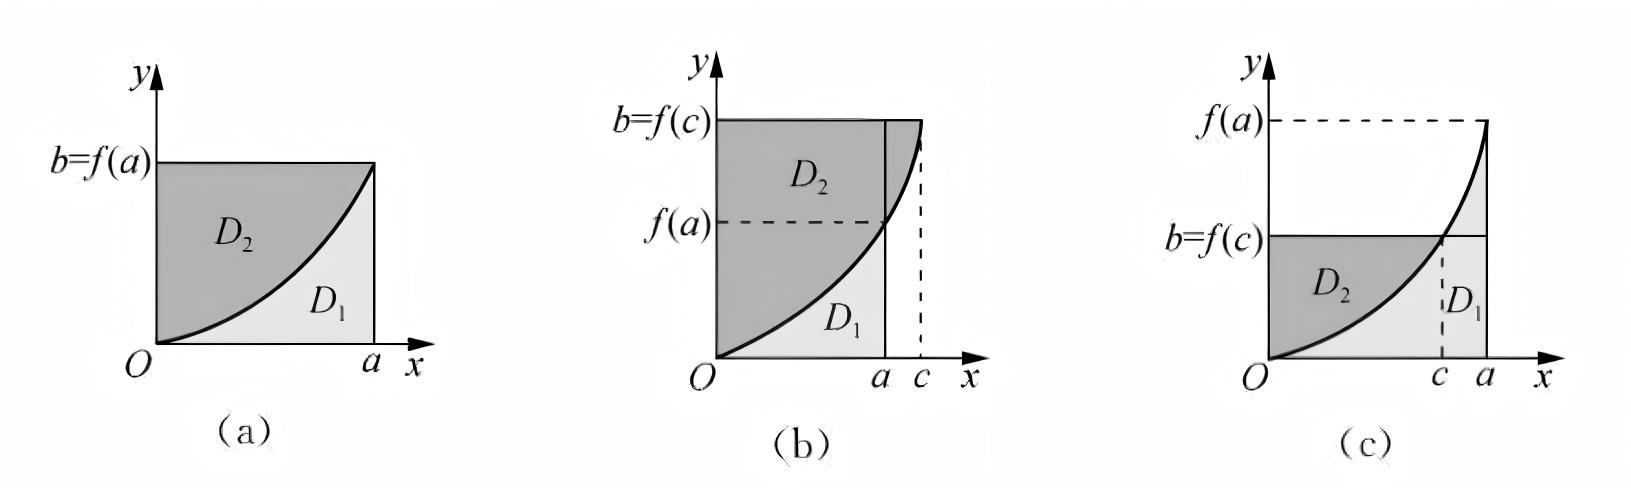
\includegraphics[width=0.7\linewidth]{figure/young}
	\end{center}
设 $f(a)=b$，取 $[0,a]$ 的划分：
	\[
	0 = x_0 < x_1 < \dots < x_n = a
	\]
	对应地令
	\[
	y_i = f(x_i)
	\]
	我们得到 $[0,b]$ 的划分
	\[
	0 = y_0 < y_1 < \dots < y_n = b
	\]
	那么
	\[
	\int_{0}^{a} f(x) \dd x = \sum_{i=1}^{n} y_{i-1} (x_i - x_{i-1}), \quad \int_{0}^{b} f^{-1}(x) \dd x = \sum_{i=1}^{n} x_i (y_i - y_{i-1})
	\]

	那么
	\begin{align*}
		\int_{0}^{a} f(x) \dd x + \int_{0}^{b} f^{-1}(x) \dd x
		&= \sum_{i=1}^{n} \left( x_i y_i - x_{i-1} y_{i-1} \right) \\
		&= x_n y_n - x_0 y_0 = ab
	\end{align*}
	
	若 $f(a) \neq b$，设 $f(T)=b$，令
	\[
	F(a) = \int_{0}^{a} f(x) \dd x + \int_{0}^{b} f^{-1}(x) \dd x - ab
	\]
	求导得
	\[
	F'(a) = f(a) - b
	\]
	
	\begin{itemize}
		\item 当 $a=T$ 时，$f(T)=b$，故 $F'(T)=0$
	 \item 当 $a>T$ 时，$f(a)>b$，故 $F'(a)>0$，$F(a)$ 单调递增
	\item 当 $a<T$ 时，$f(a)<b$，故 $F'(a)<0$，$F(a)$ 单调递减
	\end{itemize}
	
	故 $a=T$ 时 $F(a)$ 取得最小值，且 $F(T)=0$。因此 $\forall a$，有 $F(a) \geqslant 0$，也即
	\[
	\int_{0}^{a} f(x) \dd x + \int_{0}^{b} f^{-1}(x) \dd x \geqslant ab
	\]
\end{proof}
\begin{corollary}
	设 $p>1$，$q>1$ 且 $\dfrac{1}{p} + \dfrac{1}{q} = 1$，则 $\forall a,b \geqslant 0$，必有
	\[
	ab \leqslant \frac{a^p}{p} + \frac{b^q}{q}
	\]
\end{corollary}
\begin{proof}
	令 $y = x^{p-1}$，其反函数为 $x = y^{q-1}$。由Young不等式得
	\[
	\int_{0}^{a} x^{p-1} \dd x + \int_{0}^{b} x^{q-1} \dd x \geqslant ab
	\]
	计算积分即得
	\[
	ab \leqslant \frac{a^p}{p} + \frac{b^q}{q}
	\]
\end{proof}
\begin{corollary}
	（Hölder 不等式）设 $f,g \in C[a,b]$，$p,q>1$，且 $\dfrac{1}{p} + \dfrac{1}{q} = 1$，则
	\[
	\int_{a}^{b} |fg| \dd x \leqslant \left( \int_{a}^{b} |f|^p \dd x \right)^{\frac{1}{p}} \cdot \left( \int_{a}^{b} |g|^q \dd x \right)^{\frac{1}{q}}
	\]
	
若$p,q<1$，且 $\dfrac{1}{p} + \dfrac{1}{q} = 1$，则
\[
\int_{a}^{b} |fg| \dd x \geqslant \left( \int_{a}^{b} |f|^p \dd x \right)^{\frac{1}{p}} \cdot \left( \int_{a}^{b} |g|^q \dd x \right)^{\frac{1}{q}}
\]
	等号成立当且仅当$f^p(x)$与$g^q(x)$成比例时
\end{corollary}
\begin{proof}
	对任意 $\varphi(x),\psi(x) > 0$，$p,q>1$ 且 $\dfrac{1}{p} + \dfrac{1}{q} = 1$，有
	\[
	\varphi(x)\psi(x) \leqslant \frac{1}{p} \varphi(x)^p + \frac{1}{q} \psi(x)^q
	\]
	
	令
	\[
	\varphi(x) = \frac{|f(x)|}{\left( \displaystyle\int_{a}^{b} |f|^p \dd x \right)^{\frac{1}{p}}}, \quad
	\psi(x) = \frac{|g(x)|}{\left( \displaystyle\int_{a}^{b} |g|^q \dd x \right)^{\frac{1}{q}}}
	\]
	
	代入上述不等式，得
	\[
	\frac{|fg|}{\left( \displaystyle\int_{a}^{b} |f|^p \dd x \right)^{\frac{1}{p}} \left( \displaystyle\int_{a}^{b} |g|^q \dd x \right)^{\frac{1}{q}}}
	\leqslant \frac{|f|^p}{p \displaystyle\int_{a}^{b} |f|^p \dd x} + \frac{|g|^q}{q \displaystyle\int_{a}^{b} |g|^q \dd x}
	\]
	
	两边在 $[a,b]$ 上积分，整理后即得 Hölder 不等式。对称的证明类似
\end{proof}
\begin{corollary}
	(Minkowski不等式)$f,g\in\mathcal{R}[a,b]$且$f,g$的下界为正,则\[\sqrt[]{\int_{a}^{b}[f(x)+g(x)]^2\dd x}\leqslant \sqrt{\int_{a}^{b}f(x)\dd x}+\sqrt{\int_{a}^{b}g(x)\dd x}\]
\end{corollary}
\begin{proof}

	\[\begin{aligned}
			\int_{a}^{b}(f+g)^2\dd x&==2\int_{a}^{b}fg\dd x+\int_{a}^{b}f^2\dd x+\int_{a}^{b}g^2\dd x\\
			&\leqslant 2\sqrt{\int_{a}^{b}f^2\dd x\int_{a}^{b}g^2\dd x}+\int_{a}^{b}f^2\dd x+\int_{a}^{b}g^2\dd x\\
			&=(\sqrt[]{\int_{a}^{b}f^2\dd x}+\sqrt[]{\int_{a}^{b}g^2\dd x})^2
	\end{aligned}\]
\end{proof}
更进一步的，我们有
\begin{corollary}
	$f_i\in \mathcal{R}[a,b](i=1,\cdots,m)$，且下界为正，对$r>1$
	\[  \left[\int_{a}^{b}(f_1(x)+\cdots+f_m(x))^r\dd x\right]^{\frac{1}{r}}\leqslant (\int_{a}^{b}f_1^r(x)\dd x)^{\frac{1}{r}}+\cdots+(\int_{a}^{b}f_m^r(x)\dd x)^{\frac{1}{r}}  \]
	
	对$r<1$
	\[  \left[\int_{a}^{b}(f_1(x)+\cdots+f_m(x))^r\dd x\right]^{\frac{1}{r}}\geqslant (\int_{a}^{b}f_1^r(x)\dd x)^{\frac{1}{r}}+\cdots+(\int_{a}^{b}f_m^r(x)\dd x)^{\frac{1}{r}}  \]

\end{corollary}
